\documentclass{article}
\usepackage{graphicx}
\usepackage[margin=1.5cm]{geometry}
\usepackage{amsmath}
\usepackage{hyperref}

\begin{document}

\title{Week 11 Writing Activity: Writing Mechanics in Essays and Articles and Chapter 8 of \textit{The Scientific Attitude}}
\author{Prof. Jordan C. Hanson (INTD100)}

\maketitle

\section{Links for Today}
\small
\begin{enumerate}
\item
\begin{verbatim}
https://www.npr.org/2015/12/09/459026242/scientific-evidence-doesn-t-support-global-warming-sen-ted-cruz-says
\end{verbatim}
\item
\begin{verbatim}
https://www.commerce.senate.gov/2015/12/data-or-dogma-promoting-
open-inquiry-in-the-debate-over-the-magnitude-of-human-impact-on-earth-s-climate
\end{verbatim}
\item
\begin{verbatim}
https://berkeleyearth.org/guest-blog-fact-check-global-warming-pause/
\end{verbatim}
\end{enumerate}

\section{Creating an Abstract}
\normalsize
Imagine an experiment where you measure the density of an object my submerging it in water, and then weighing it.  Write an abstract describing the results.  You would first measure the volume of an object by submerging it and measuring the increase in water level.  Second, you would form a ratio of the mass divided by the volume to give the density.

\section{Pseudo-Science and Denialism}

\begin{enumerate}
\item Let's have a discussion about the junctures in the above debates in which \textit{denialism} enters.  By the way, it is perfectly fine to have questions about the scientific evidence, and to be skeptical.  Is your skepticism reasonable, given what we have encountered in Ch. 8 of the book? \\ \vspace{2cm}
\item Recall the story of J. Harlen Bretz, the geologist who first predicted the glacial flood that shaped the channeled scablands of Washington State.  Was Bretz an example of a denialist, or were his colleagues in the \textit{uniformitarian} school of thought?
\end{enumerate}
\small
\begin{figure}
\centering
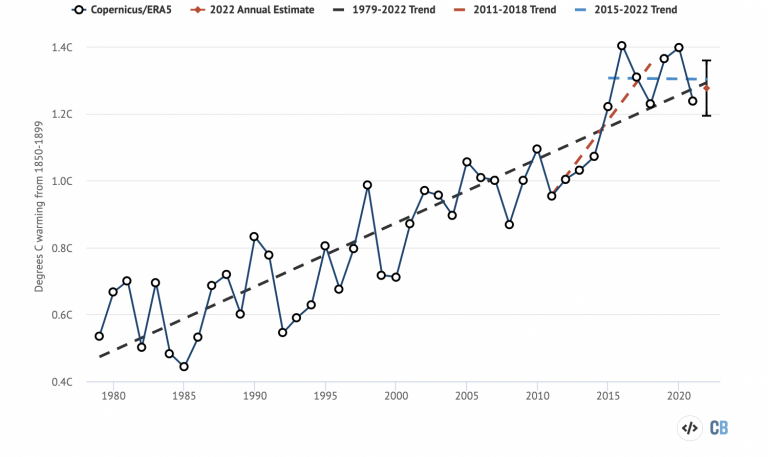
\includegraphics[width=0.45\textwidth]{figures/pause.png}
\caption{\label{fig:1} Source: Z. HausFather, Berkeley Earth Project.}
\end{figure}

\end{document}
